\begin{figure}[htbp]
    \centering
    % First TikZ picture
    \begin{subfigure}[b]{0.45\textwidth}
        \centering
        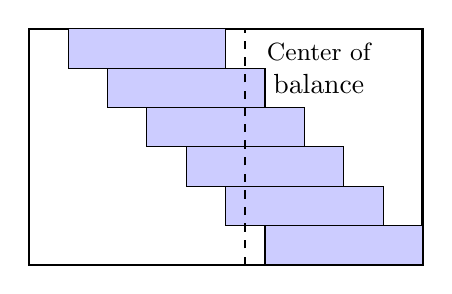
\begin{tikzpicture}
            % Draw the container
            \draw[thick] (0,0) rectangle (5,3);

            % Draw the three items inside
            \draw[fill=blue!20] (3,0) rectangle (5,0.5);
            \draw[fill=blue!20] (2.5,0.5) rectangle (4.5,1);
            \draw[fill=blue!20] (2,1) rectangle (4, 1.5);
            \draw[fill=blue!20] (1.5,1.5) rectangle (3.5, 2);
            \draw[fill=blue!20] (1,2) rectangle (3, 2.5);
            \draw[fill=blue!20] (0.5,2.5) rectangle (2.5, 3);
            %\node at (4, 1.875) {Fragile};
            \draw[thick,dashed] (2.75,0) -- (2.75,3);  % <---
            \node[anchor = west,align=center] at (2.9,2.5) {\small Center of \\  balance};

        \end{tikzpicture}
        \caption[align = center]{Feasible stacking with 75\% support area; infeasible due to unstable center}
    \end{subfigure}
    \hfill
    % Second TikZ picture
    \begin{subfigure}[b]{0.45\textwidth}
        \centering
        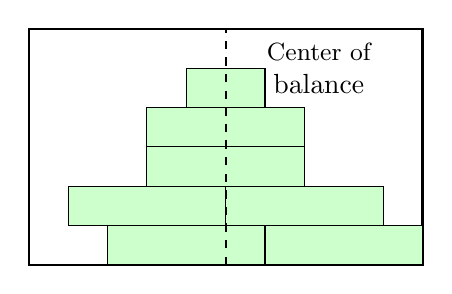
\begin{tikzpicture}
            % Draw the container
            \draw[thick] (0,0) rectangle (5,3);

            % Draw the three items inside
            \draw[fill=green!20] (3,0) rectangle (5,0.5);
            \draw[fill=green!20] (1,0) rectangle (3,0.5);

            \draw[fill=green!20] (2.5,0.5) rectangle (4.5,1);
            \draw[fill=green!20] (0.5,0.5) rectangle (2.5,1);

            \draw[fill=green!20] (1.5,1) rectangle (3.5, 1.5);
            \draw[fill=green!20] (1.5,1.5) rectangle (3.5, 2);
            \draw[fill=green!20] (2,2) rectangle (3, 2.5);

            \draw[thick,dashed] (2.5,0) -- (2.5,3);  % <---
            \node[anchor = west,align=center] at (2.9,2.5) {\small Center of \\  balance};
        \end{tikzpicture}
        \caption[align = center]{Feasible stacking regarding 75\% support area and stable center}
    \end{subfigure}
    \caption[Comparison of different vertical stability constraints]{Comparison of different vertical stability constraints (side view) \footnotemark}
    \footnotetext{Own figures based on \cite[p.845]{krebs_advanced_2021}}
    \label{fig:vertical_stability_comparison}
\end{figure}
